%===============================================================================
% LaTeX sjabloon voor de bachelorproef toegepaste informatica aan HOGENT
% Meer info op https://github.com/HoGentTIN/latex-hogent-report
%===============================================================================

\documentclass[dutch,dit,thesis]{hogentreport}

% TODO:
% - If necessary, replace the option `dit`' with your own department!
%   Valid entries are dbo, dbt, dgz, dit, dlo, dog, dsa, soa
% - If you write your thesis in English (remark: only possible after getting
%   explicit approval!), remove the option "dutch," or replace with "english".

\usepackage{lipsum} % For blind text, can be removed after adding actual content

%% Pictures to include in the text can be put in the graphics/ folder
\graphicspath{{graphics/}}

%% For source code highlighting, requires pygments to be installed
%% Compile with the -shell-escape flag!
\usepackage[section]{minted}
%% If you compile with the make_thesis.{bat,sh} script, use the following
%% import instead:
%% \usepackage[section,outputdir=../output]{minted}
\usemintedstyle{solarized-light}
\definecolor{bg}{RGB}{253,246,227} %% Set the background color of the codeframe

%% Change this line to edit the line numbering style:
\renewcommand{\theFancyVerbLine}{\ttfamily\scriptsize\arabic{FancyVerbLine}}

%% Macro definition to load external java source files with \javacode{filename}:
\newmintedfile[javacode]{java}{
    bgcolor=bg,
    fontfamily=tt,
    linenos=true,
    numberblanklines=true,
    numbersep=5pt,
    gobble=0,
    framesep=2mm,
    funcnamehighlighting=true,
    tabsize=4,
    obeytabs=false,
    breaklines=true,
    mathescape=false
    samepage=false,
    showspaces=false,
    showtabs =false,
    texcl=false,
}

% Other packages not already included can be imported here

%%---------- Document metadata -------------------------------------------------
% TODO: Replace this with your own information
\author{Ernst Aarden}
\supervisor{Dhr. F. Van Houte}
\cosupervisor{Mevr. S. Beeckman}
\title[Optionele ondertitel]%
    {Titel van de bachelorproef}
\academicyear{\advance\year by -1 \the\year--\advance\year by 1 \the\year}
\examperiod{1}
\degreesought{\IfLanguageName{dutch}{Professionele bachelor in de toegepaste informatica}{Bachelor of applied computer science}}
\partialthesis{false} %% To display 'in partial fulfilment'
%\institution{Internshipcompany BVBA.}

%% Add global exceptions to the hyphenation here
\hyphenation{back-slash}

%% The bibliography (style and settings are  found in hogentthesis.cls)
\addbibresource{bachproef.bib}            %% Bibliography file
\addbibresource{../voorstel/voorstel.bib} %% Bibliography research proposal
\defbibheading{bibempty}{}

%% Prevent empty pages for right-handed chapter starts in twoside mode
\renewcommand{\cleardoublepage}{\clearpage}

\renewcommand{\arraystretch}{1.2}

%% Content starts here.
\begin{document}

%---------- Front matter -------------------------------------------------------

\frontmatter

\hypersetup{pageanchor=false} %% Disable page numbering references
%% Render a Dutch outer title page if the main language is English
\IfLanguageName{english}{%
    %% If necessary, information can be changed here
    \degreesought{Professionele Bachelor toegepaste informatica}%
    \begin{otherlanguage}{dutch}%
       \maketitle%
    \end{otherlanguage}%
}{}

%% Generates title page content
\maketitle
\hypersetup{pageanchor=true}

%%=============================================================================
%% Voorwoord
%%=============================================================================

\chapter*{\IfLanguageName{dutch}{Woord vooraf}{Preface}}%
\label{ch:voorwoord}

%% TODO:
%% Het voorwoord is het enige deel van de bachelorproef waar je vanuit je
%% eigen standpunt (``ik-vorm'') mag schrijven. Je kan hier bv. motiveren
%% waarom jij het onderwerp wil bespreken.
%% Vergeet ook niet te bedanken wie je geholpen/gesteund/... heeft



Ik wil dit onderwerp bespreken omdat Garbage Collection in Java wel een brede onderwerp is dat nog steeds relevant blijkt tot vandaag de dag, het leek mij ook interessant omdat deze thema toch ook wel zeer diepgaand is, in de zin dat het zeer \textit{low-level} gaat, en ook een groot deel theoretische computerwetenschap is.
Verder nog vind ik het zeer interessant om over de mainframe te kunnen spreken, het is een grootschalig thema die vandaag de dag eerder in de schaduw ligt.
Zelf ben ik zeer blij dat ik in de mainframe niche ben getrokken, het is een rijke en boeiende wereld waarin ik nog veel te leren heb.



Vanuit HOGENT zou ik graag mijn promoter, Sion Verschraege bedanken voor de telkens spoedige feedback en beschikbaarheid, en Leendert Blondeel voor het oprichten van de mainframe expert keuzetraject.


Ik wil mijn co-promoter, Jan Cannaerts bedanken voor de hulp in het mogelijk maken om de Java programma's te kunnen laten werken op mainframe, en voor het theoretisch uitleg hieromtrent.
Alsook wil ik Solidaris bedanken voor de mogelijkheid om hun mainframes te kunnen gebruiken om mijn testen uit te voeren.


Ik zou ook graag mijn vader, Johan Briké, mijn moeder Jadranka Briké, en mijn vriendin Vaneeda Vermeersch bedanken voor hun steun.

Verder nog zou ik graag Mathias De Gryse en Michael Liu bedanken voor hun taalkundig hulp te bieden.



%%=============================================================================
%% Samenvatting
%%=============================================================================

% TODO: De "abstract" of samenvatting is een kernachtige (~ 1 blz. voor een
% thesis) synthese van het document.
%
% Een goede abstract biedt een kernachtig antwoord op volgende vragen:
%
% 1. Waarover gaat de bachelorproef?
% 2. Waarom heb je er over geschreven?
% 3. Hoe heb je het onderzoek uitgevoerd?
% 4. Wat waren de resultaten? Wat blijkt uit je onderzoek?
% 5. Wat betekenen je resultaten? Wat is de relevantie voor het werkveld?
%
% Daarom bestaat een abstract uit volgende componenten:
%
% - inleiding + kaderen thema
% - probleemstelling
% - (centrale) onderzoeksvraag
% - onderzoeksdoelstelling
% - methodologie
% - resultaten (beperk tot de belangrijkste, relevant voor de onderzoeksvraag)
% - conclusies, aanbevelingen, beperkingen
%
% LET OP! Een samenvatting is GEEN voorwoord!

%%---------- Nederlandse samenvatting -----------------------------------------
%
% TODO: Als je je bachelorproef in het Engels schrijft, moet je eerst een
% Nederlandse samenvatting invoegen. Haal daarvoor onderstaande code uit
% commentaar.
% Wie zijn bachelorproef in het Nederlands schrijft, kan dit negeren, de inhoud
% wordt niet in het document ingevoegd.

\IfLanguageName{english}{%
\selectlanguage{dutch}
\chapter*{Samenvatting}
\lipsum[1-4]
\selectlanguage{english}
}{}

%%---------- Samenvatting -----------------------------------------------------
% De samenvatting in de hoofdtaal van het document

\chapter*{\IfLanguageName{dutch}{Samenvatting}{Abstract}}

\lipsum[1-4]


%---------- Inhoud, lijst figuren, ... -----------------------------------------

\tableofcontents

% In a list of figures, the complete caption will be included. To prevent this,
% ALWAYS add a short description in the caption!
%
%  \caption[short description]{elaborate description}
%
% If you do, only the short description will be used in the list of figures

\listoffigures

% If you included tables and/or source code listings, uncomment the appropriate
% lines.
%\listoftables
%\listoflistings

% Als je een lijst van afkortingen of termen wil toevoegen, dan hoort die
% hier thuis. Gebruik bijvoorbeeld de ``glossaries'' package.
% https://www.overleaf.com/learn/latex/Glossaries

%---------- Kern ---------------------------------------------------------------

\mainmatter{}

% De eerste hoofdstukken van een bachelorproef zijn meestal een inleiding op
% het onderwerp, literatuurstudie en verantwoording methodologie.
% Aarzel niet om een meer beschrijvende titel aan deze hoofdstukken te geven of
% om bijvoorbeeld de inleiding en/of stand van zaken over meerdere hoofdstukken
% te verspreiden!

%%=============================================================================
%% Inleiding
%%=============================================================================

\chapter{\IfLanguageName{dutch}{Inleiding}{Introduction}}%
\label{ch:inleiding}

%De inleiding moet de lezer net genoeg informatie verschaffen om het onderwerp te begrijpen en in te zien waarom de onderzoeksvraag de moeite waard is om te onderzoeken. In de inleiding ga je literatuurverwijzingen beperken, zit de tekst vlot leesbaar blijft. Je kan de inleiding verder onderverdelen in secties als dit de tekst verduidelijkt. Zaken die aan bod kunnen komen in de inleiding~\autocite{Pollefliet2011}:


\section{\IfLanguageName{dutch}{Probleemstelling}{Problem Statement}}%
\label{sec:probleemstelling}

%Uit je probleemstelling moet duidelijk zijn dat je onderzoek een meerwaarde heeft voor een concrete doelgroep. De doelgroep moet goed gedefinieerd en afgelijnd zijn. Doelgroepen als ``bedrijven,'' ``KMO's'', systeembeheerders, enz.~zijn nog te vaag. Als je een lijstje kan maken van de personen/organisaties die een meerwaarde zullen vinden in deze bachelorproef (dit is eigenlijk je steekproefkader), dan is dat een indicatie dat de doelgroep goed gedefinieerd is. Dit kan een enkel bedrijf zijn of zelfs één persoon (je co-promotor/opdrachtgever).


\let\oldquote\quote
\let\endoldquote\endquote
\renewenvironment{quote}[2][]
{\if\relax\detokenize{#1}\relax
    \def\quoteauthor{#2}%
    \else
    \def\quoteauthor{#2~---~#1}%
    \fi
    \oldquote}
{\par\nobreak\smallskip\hfill(\quoteauthor)%
    \endoldquote\addvspace{\bigskipamount}}

Bedrijven die gebruik maken van een mainframe kunnen baat hebben bij het maken van Java programma's voor mainframe, of het migreren van bestaande Java programma's naar mainframe.
Er zijn meerdere redenen waarom dit een voordeel kan bieden, de voornaamste zijn:
    \begin{itemize}
    \item Een mainframe is gemaakt om zeer veel transacties te kunnen verwerken, Java programma's die grote hoeveelheden data moeten verwerken kunnen dus de mainframe hiervoor gebruiken.
    \item De mainframe maakt gebruik van technologieën en programmeertalen die al ontworpen zijn sinds de eerste generaties van mainframes.
     Zoals \textit{COBOL} uit 1959 of \textit{Job Control Language} uit 1964 die beschreven werd door de uitvinder als;
    \begin{quote}{Fred Brooks}
        Job Control Language is the worst programming language ever designed anywhere by anybody for any purpose.
    \end{quote}}
    Het is noodzakelijk dat de mainframe compatibel blijft met oude programma's, deze zijn geschreven in programmeertalen die vandaag de dag als ouderwets beschouwd worden, en niet meer aangeleerd worden door de nieuwe generaties van IT'ers.
    Daarom dat Java op mainframe gebruiken interessant is omdat er een groter aantal mensen bekwaam zijn met deze programmeertaal in vergelijking met de traditionele mainframe programmeertalen, zoals onder andere PL/I, COBOL, Assembler of CICS.
    
    
    \item Java programma's die op mainframe draaien worden via de zIIP processor verwerkt, dit brengt ook enkele voordelen, dit onderwerp zal in de methodologie verder verbreed worden.
    
    
 \end{itemize}
\section{\IfLanguageName{dutch}{Onderzoeksvraag}{Research question}}%
\label{sec:onderzoeksvraag}

%Wees zo concreet mogelijk bij het formuleren van je onderzoeksvraag. Een onderzoeksvraag is trouwens iets waar nog niemand op dit moment een antwoord heeft (voor zover je kan nagaan). Het opzoeken van bestaande informatie (bv. ``welke tools bestaan er voor deze toepassing?'') is dus geen onderzoeksvraag. Je kan de onderzoeksvraag verder specifiëren in deelvragen. Bv.~als je onderzoek gaat over performantiemetingen, dan 
De onderzoeksvraag van deze thesis is 'Wat zijn de gevolgen voor Garbage Collection bij het migreren van Java programma's naar mainframe?'.
Hieruit kunnen we ook enkele deelvragen stellen.

\begin{itemize}
    \item Is Garbage Collection voor Java op niet-mainframe en mainframe gelijkaardig qua performantie?
    \item Wat is de invloed van Garbage Collection in Java op niet-mainframe en op mainframe qua efficiëntie?
    \item Werkt een Garbage Collector qua performantie hetzelfde wanneer er een programma van niet-mainframe naar mainframe migreert wordt?
\end{itemize}



  

\section{\IfLanguageName{dutch}{Onderzoeksdoelstelling}{Research objective}}%
\label{sec:onderzoeksdoelstelling}

De doelstelling van dit onderzoek is om een vergelijkende studie te maken omtrent de werking van Garbage Collection op mainframe en niet-mainframe.
Dit door het vergelijken van een aantal statistieken verkregen vanuit testprogramma's.


%Wat is het beoogde resultaat van je bachelorproef? Wat zijn de criteria voor succes? Beschrijf die zo concreet mogelijk. Gaat het bv.\ om een proof-of-concept, een prototype, een verslag met aanbevelingen, een vergelijkende studie, enz.

\section{\IfLanguageName{dutch}{Opzet van deze bachelorproef}{Structure of this bachelor thesis}}%
\label{sec:opzet-bachelorproef}

% Het is gebruikelijk aan het einde van de inleiding een overzicht te
% geven van de opbouw van de rest van de tekst. Deze sectie bevat al een aanzet
% die je kan aanvullen/aanpassen in functie van je eigen tekst.

De rest van deze bachelorproef is als volgt opgebouwd:

In Hoofdstuk~\ref{ch:stand-van-zaken} wordt een overzicht gegeven van de stand van zaken binnen het onderzoeksdomein, op basis van een literatuurstudie.

In Hoofdstuk~\ref{ch:methodologie} wordt de methodologie toegelicht en worden de gebruikte onderzoekstechnieken besproken om een antwoord te kunnen formuleren op de onderzoeksvragen.

% TODO: Vul hier aan voor je eigen hoofstukken, één of twee zinnen per hoofdstuk

In Hoofdstuk~\ref{ch:uitvoering} wordt de effectieve uitvoering van de testen besproken.

In Hoofdstuk~\ref{ch:analyse} wordt de bekomen data gegeven en toegelicht.

In Hoofdstuk~\ref{ch:conclusie}, tenslotte, wordt de conclusie gegeven en een antwoord geformuleerd op de onderzoeksvragen. Daarbij wordt ook een aanzet gegeven voor toekomstig onderzoek binnen dit domein.
\chapter{\IfLanguageName{dutch}{Stand van zaken}{State of the art}}%
\label{ch:stand-van-zaken}

% Tip: Begin elk hoofdstuk met een paragraaf inleiding die beschrijft hoe
% dit hoofdstuk past binnen het geheel van de bachelorproef. Geef in het
% bijzonder aan wat de link is met het vorige en volgende hoofdstuk.

% Pas na deze inleidende paragraaf komt de eerste sectiehoofding.

Dit hoofdstuk bevat je literatuurstudie. De inhoud gaat verder op de inleiding, maar zal het onderwerp van de bachelorproef *diepgaand* uitspitten. De bedoeling is dat de lezer na lezing van dit hoofdstuk helemaal op de hoogte is van de huidige stand van zaken (state-of-the-art) in het onderzoeksdomein. Iemand die niet vertrouwd is met het onderwerp, weet nu voldoende om de rest van het verhaal te kunnen volgen, zonder dat die er nog andere informatie moet over opzoeken \autocite{Pollefliet2011}.

Je verwijst bij elke bewering die je doet, vakterm die je introduceert, enz.\ naar je bronnen. In \LaTeX{} kan dat met het commando \texttt{$\backslash${textcite\{\}}} of \texttt{$\backslash${autocite\{\}}}. Als argument van het commando geef je de ``sleutel'' van een ``record'' in een bibliografische databank in het Bib\LaTeX{}-formaat (een tekstbestand). Als je expliciet naar de auteur verwijst in de zin (narratieve referentie), gebruik je \texttt{$\backslash${}textcite\{\}}. Soms is de auteursnaam niet expliciet een onderdeel van de zin, dan gebruik je \texttt{$\backslash${}autocite\{\}} (referentie tussen haakjes). Dit gebruik je bv.~bij een citaat, of om in het bijschrift van een overgenomen afbeelding, broncode, tabel, enz. te verwijzen naar de bron. In de volgende paragraaf een voorbeeld van elk.

\textcite{Knuth1998} schreef een van de standaardwerken over sorteer- en zoekalgoritmen. Experten zijn het erover eens dat cloud computing een interessante opportuniteit vormen, zowel voor gebruikers als voor dienstverleners op vlak van informatietechnologie~\autocite{Creeger2009}.

Let er ook op: het \texttt{cite}-commando voor de punt, dus binnen de zin. Je verwijst meteen naar een bron in de eerste zin die erop gebaseerd is, dus niet pas op het einde van een paragraaf.

\lipsum[7-20]

%%=============================================================================
%% Methodologie
%%=============================================================================

\chapter{\IfLanguageName{dutch}{Methodologie}{Methodology}}%
\label{ch:methodologie}

%% TODO: In dit hoofstuk geef je een korte toelichting over hoe je te werk bent
%% gegaan. Verdeel je onderzoek in grote fasen, en licht in elke fase toe wat
%% de doelstelling was, welke deliverables daar uit gekomen zijn, en welke
%% onderzoeksmethoden je daarbij toegepast hebt. Verantwoord waarom je
%% op deze manier te werk gegaan bent.
%% 
%% Voorbeelden van zulke fasen zijn: literatuurstudie, opstellen van een
%% requirements-analyse, opstellen long-list (bij vergelijkende studie),
%% selectie van geschikte tools (bij vergelijkende studie, "short-list"),
%% opzetten testopstelling/PoC, uitvoeren testen en verzamelen
%% van resultaten, analyse van resultaten, ...
%%
%% !!!!! LET OP !!!!!
%%
%% Het is uitdrukkelijk NIET de bedoeling dat je het grootste deel van de corpus
%% van je bachelorproef in dit hoofstuk verwerkt! Dit hoofdstuk is eerder een
%% kort overzicht van je plan van aanpak.
%%
%% Maak voor elke fase (behalve het literatuuronderzoek) een NIEUW HOOFDSTUK aan
%% en geef het een gepaste titel.




\chapter{Opstelling}

\chapter{Uitvoering}

\chapter{Analyse}

% Voeg hier je eigen hoofdstukken toe die de ``corpus'' van je bachelorproef
% vormen. De structuur en titels hangen af van je eigen onderzoek. Je kan bv.
% elke fase in je onderzoek in een apart hoofdstuk bespreken.

%\input{...}
%\input{...}
%...

%%=============================================================================
%% Conclusie
%%=============================================================================

\chapter{Conclusie}%
\label{ch:conclusie}

% TODO: Trek een duidelijke conclusie, in de vorm van een antwoord op de
% onderzoeksvra(a)g(en). Wat was jouw bijdrage aan het onderzoeksdomein en
% hoe biedt dit meerwaarde aan het vakgebied/doelgroep? 
% Reflecteer kritisch over het resultaat. In Engelse teksten wordt deze sectie
% ``Discussion'' genoemd. Had je deze uitkomst verwacht? Zijn er zaken die nog
% niet duidelijk zijn?
% Heeft het onderzoek geleid tot nieuwe vragen die uitnodigen tot verder 
%onderzoek?




%todo beter maken 
We kunnen opmerken dat er een degelijke verschil is aan data tussen de programma's, er is geen enkel garbage Collector dat voor elk programma het beste uitschijnt.
Het is noodzakelijk om voor elk individueel programma na te kijken wat de beste Garbage Collector blijkt te zijn.


De bekomen data voor de gencon policy met \textit{ConcurrentScavenge} blijkt niet overweldigend beter te zijn voor mainframe in vergelijking met niet-mainframe, dit ondanks de hardware geassisteerde \textit{Pause-less Garbage Collection} voor de IBM mainframes.
Zelfs blijkt dat de gencon policy zonder ConcurrentScavenge op mainframe soms gelijk of zelfs beter blijkt de werken dan de gencon policy met \textit{ConcurrentScavenge}.


Er blijkt ook dat er een verschil in werking kan zijn tussen Garbage Collectors op mainframe en niet-mainframe, dit is meest duidelijk te zien aan de totale pauzetijd tussen de optavgpause en optthruput policies voor finagle-chirper, waarbij de optavgpause meer totale pauzetijd heeft voor niet-mainframe, maar voor mainframe heeft de optthruput meer totale pauzetijd.

Dit betekent dat het voor het migreren van een programma van niet-mainframe naar mainframe, of vice-versa, het nog steeds noodzakelijk is om opnieuw onderzoek te doen naar de optimale garbage Collection policy voor het nieuw systeem, en dat het niet noodzakelijk de beste optie is om de al voorheen gebruikte Garbage Collection policy over te nemen.

%---------- Bijlagen -----------------------------------------------------------

\appendix

\chapter{Onderzoeksvoorstel}

Het onderwerp van deze bachelorproef is gebaseerd op een onderzoeksvoorstel dat vooraf werd beoordeeld door de promotor. Dat voorstel is opgenomen in deze bijlage.

%% TODO: 
%\section*{Samenvatting}

% Kopieer en plak hier de samenvatting (abstract) van je onderzoeksvoorstel.

% Verwijzing naar het bestand met de inhoud van het onderzoeksvoorstel
%---------- Inleiding ---------------------------------------------------------

\section{Introductie}%
\label{sec:introductie}
%De prestatie van een programma is een van de belangrijkste aspecten van het ontwikkelen van eender welk software, in deze onderzoek zal voornamelijk de geheugengebruik en totale uitvoeringstijd van de Garbage Collection van de applicatie gemeten worden.
Dit onderzoek zal zich verdiepen op welke invloed Garbage Collection heeft op de prestatie van Java programma's, specifieker voor programma's die naar mainframe gemigreerd worden.
De geheugengebruik en totale uitvoeringstijd van de Garbage Collection van de applicatie zal gemeten worden en gebruikt worden voor de vergelijkingen.

Garbage Collection is een essentieel onderdeel van Java, het ruimt onnodige objecten op in het geheugen om het weer vrij te maken.

De centrale onderzoeksvraag is 'Welke invloed heeft het migreren naar mainframe van Java programma's op Garbage Collection?'.
Er zijn bepaalde deelvragen die zullen uitgewerkt worden, namelijk:

\begin{enumerate}
    \item Wat zijn de criteria om te bepalen welke Garbage Collector de beste performantie oplevert voor een programma? 
    \item Is er een correlatie tussen Garbage Collection op niet-mainframe systemen en mainframes, en tussen Z/OS en zLinux?
    \item Hoe werkt de IBM Pause-less Garbage Collector? 
    \item Welke parameters kunnen we veranderen aan de Garbage Collectors, en met welke gevolgen? 
    \item Wat zijn de verschillende use cases voor de verschillende Garbage Collectors?  
\end{enumerate}

Aan het eind van dit onderzoek zal blijken als er een correlatie is tussen Garbage collection voor Java programma's op mainframe en Java programma's niet op mainframe.
Alsook zal er blijken wat de mogelijkheden zijn om een Java programma op mainframe beter te laten presteren door de gebruikte Garbage Collector te veranderen, en, of hem aan te passen via aanpasbare parameters, zoals de \textit{-Xmx} parameter om de maximale heap geheugen in te stellen, en de \textit{-XX:MaxGCPauseMillis} parameter om de maximale pauzetijd van de Garbage Collector in te stellen.


%Waarover zal je bachelorproef gaan? Introduceer het thema en zorg dat volgende zaken zeker duidelijk aanwezig zijn:

%\begin{itemize}
%  \item kaderen thema
%  \item de doelgroep
%  \item de probleemstelling en (centrale) onderzoeksvraag
%  \item de onderzoeksdoelstelling
%\end{itemize}

%Denk er aan: een typische bachelorproef is \textit{toegepast onderzoek}, wat betekent dat je start vanuit een concrete probleemsituatie in bedrijfscontext, een \textbf{casus}. Het is belangrijk om je onderwerp goed af te bakenen: je gaat voor die \textit{ene specifieke probleemsituatie} op zoek naar een goede oplossing, op basis van de huidige kennis in het vakgebied.

%De doelgroep moet ook concreet en duidelijk zijn, dus geen algemene of vaag gedefinieerde groepen zoals \emph{bedrijven}, \emph{developers}, \emph{Vlamingen}, enz. Je richt je in elk geval op it-professionals, een bachelorproef is geen populariserende tekst. Eén specifiek bedrijf (die te maken hebben met een concrete probleemsituatie) is dus beter dan \emph{bedrijven} in het algemeen.

%Formuleer duidelijk de onderzoeksvraag! De begeleiders lezen nog steeds te veel voorstellen waarin we geen onderzoeksvraag terugvinden.

%Schrijf ook iets over de doelstelling. Wat zie je als het concrete eindresultaat van je onderzoek, naast de uitgeschreven scriptie? Is het een proof-of-concept, een rapport met aanbevelingen, \ldots Met welk eindresultaat kan je je bachelorproef als een succes beschouwen?

%---------- Stand van zaken ---------------------------------------------------

\section{State-of-the-art}%
\label{sec:state-of-the-art}

Garbage Collection is een essentieel onderdeel van Java, het maakt automatisch geheugenbeheer mogelijk waardoor de ontwikkelaar niet zelf expliciet het geheugen moet beheren in zijn programma.
Het hoofdprincipe van de automatische geheugenbeheer in Java is om het geheugen van objecten waarnaar niet meer in de \textit{heap} geheugen verwezen wordt te herstellen en terug te voorzien.
Het is mogelijk om met de \textit{System.gc()} methode een expliciete aanvraag voor Garbage Collection te versturen naar de JVM, maar als er niet voldoende geheugen is om Garbage Collection uit te voeren zal de JVM dit ook niet doen.


Het Heap geheugen is een deel van het geheugen dat aangemaakt wordt bij het opstarten van de Java Virtual machine (JVM), deze wordt gebruikt om geheugen aan alle objecten en arrays toe te wijzen.
Verder is er nog de Stack geheugen, deze wordt gebruikt om geheugen toe te wijzen aan lokale variabelen binnenin methodes, wanneer een methode wordt opgeroepen wordt er een nieuw blok voorzien voor deze methode in de Stack geheugen waarin de variabelen voor deze methode opgeslagen worden \autocite{Cavanna2003}.
Eens de methode is afgewerkt zal deze blok uit de Stack geheugen verwijderd worden.
Alle JVM threads kunnen toegang tot de objecten in het heap geheugen krijgen, alsook toewijzingen uitvoeren zolang er nog voldoende geheugen beschikbaar is. 

Garbage verwijst naar objecten in het heap geheugen waarnaar geen andere objecten meer naar verwijzen, deze objecten mogen verwijderd worden.

Tijdens het uitvoeren van de Garbage Collection worden alle niet essentiële threads gepauzeerd, dit wordt een Stop-The-World event genoemd, enkel nadat de Garbage Collection processen klaar zijn zullen de onderbroken threads verder uitgevoerd worden\autocite{Grgic2018}.

Met de Z14 mainframe heeft IBM een nieuwe facilitet voorzien, de \textit{Guarded-Storage Facility}.
Volgens \textcite{Gracie} kan door het gebruik van de Gaurded Storage Faclity om bepaalde regio's van geheugen op te slaan het mogelijk zijn om maar een korte \textit{Stop The World event} aan het begin en einde van de Garbage Collection te hebben, en niet gedurende de gehele Garbage Collection.

Door onderzoek naar Garbage Collection, waaronder \textcite{Bruno2018} en \textcite{Nguyen2016} merken we dat er nog steeds nood is aan verder onderzoek in dit veld, en dat het een reëel probleem voorstelt.




%Hier beschrijf je de \emph{state-of-the-art} rondom je gekozen onderzoeksdomein, d.w.z.\ een inleidende, doorlopende tekst over het onderzoeksdomein van je bachelorproef. Je steunt daarbij heel sterk op de professionele \emph{vakliteratuur}, en niet zozeer op populariserende teksten voor een breed publiek. Wat is de huidige stand van zaken in dit domein, en wat zijn nog eventuele open vragen (die misschien de aanleiding waren tot je onderzoeksvraag!)?

%Je mag de titel van deze sectie ook aanpassen (literatuurstudie, stand van zaken, enz.). Zijn er al gelijkaardige onderzoeken gevoerd? Wat concluderen ze? Wat is het verschil met jouw onderzoek?

%Verwijs bij elke introductie van een term of bewering over het domein naar de vakliteratuur, bijvoorbeeld~\autocite{Hykes2013}! Denk zeker goed na welke werken je refereert en waarom.

%Draag zorg voor correcte literatuurverwijzingen! Een bronvermelding hoort thuis \emph{binnen} de zin waar je je op die bron baseert, dus niet er buiten! Maak meteen een verwijzing als je gebruik maakt van een bron. Doe dit dus \emph{niet} aan het einde van een lange paragraaf. Baseer nooit teveel aansluitende tekst op eenzelfde bron.

%Als je informatie over bronnen verzamelt in JabRef, zorg er dan voor dat alle nodige info aanwezig is om de bron terug te vinden (zoals uitvoerig besproken in de lessen Research Methods).

% Voor literatuurverwijzingen zijn er twee belangrijke commando's:
% \autocite{KEY} => (Auteur, jaartal) Gebruik dit als de naam van de auteur
%   geen onderdeel is van de zin.
% \textcite{KEY} => Auteur (jaartal)  Gebruik dit als de auteursnaam wel een
%   functie heeft in de zin (bv. ``Uit onderzoek door Doll & Hill (1954) bleek
%   ...'')

%Je mag deze sectie nog verder onderverdelen in subsecties als dit de structuur van de tekst kan verduidelijken.

%---------- Methodologie ------------------------------------------------------
\section{Methodologie}%
\label{sec:methodologie}


Eerst zal er een literatuurstudie gedaan worden naar de werking van de Garbage Collectors, de theoretische algoritmen waarop ze steunen, de verschillende fases in Garbage Collection, de algemene kenmerken en de individuele verschillen van de gekozen Garbage Collectors.
De Garbage Collectors zullen gekozen worden aan de hand van bepaalde criteria, namelijk de leeftijd, de beherende organisatie waarvan het afkomstig is, en de al dan niet al onderzochte prestatie.

Vervolgens zullen we enkele Java benchmarks uitvoeren op mainframe en niet-mainframe, deze zullen ons met data over de Garbage Collection geven, zoals het geheugengebruik en de duur van tijd er gepauzeerd wordt voor Garbage Collection.

Eens we deze benchmarks hebben uitgevoerd zullen we over alle nodige data beschikken om onze onderzoek naar de Garbage Collection prestaties uit te voeren.
We zullen de verschillende Garbage Collection algoritmes vergelijken, hun correlatie tussen mainframe en niet-mainframe, en de invloed van de verschillende parameters die we hebben aangepast
Aan de hand hiervan kunnen we een conclusie bekomen.

De DaCapo\footnote{https://dacapo-bench.org/} benchmark suite geeft ons de mogelijkheid om enkele real-world Java applicaties te gebruiken.
Aan de hand van deze applicaties is het mogelijk om een grote waaier van verschillende use cases te vergelijken.
Deze applicaties krijgen telkens via de applicatie zelve dezelfde input, dit zorgt ervoor dat er geen menselijke input verwacht wordt waardoor er mogelijk niet objectieve metingen ontstaan.
Door dezelfde applicaties op mainframe en niet mainframe te gebruiken kunnen we de migratie van programma's naar mainframe simuleren.
We zullen de Java applicaties begrenzen door verschillende parameters mee te geven, zoals \textit{-Xss} voor de stack size te bepalen.
Hierdoor garanderen we dat de uitvoering van de programma's op mainframe en niet mainframe niet beïnvloed wordt door verschillen in de capaciteit van de systemen.

Om de Java applicaties te laten draaien kunnen we gebruik maken van een mainframe die Z/OS draait, deze mainframe zal minstens de Z14 model moeten zijn om gebruik te kunnen maken van de Pause-less Garbage Collection.
Het kan ook interessant zijn om het in een zLinux omgeving te draaien, om eventuele verschillen op te merken, de Hercules\footnote{http://www.hercules-390.org/} z/Architecture Emulator kunnen we gebruiken om te zien wat de impact is van de applicaties niet op mainframe zelf te draaien.

Er zijn bepaalde metrieken die wij kunnen opmeten om een vergelijking tussen de Garbage Collectors te kunnen maken, voornamelijk is dit:
\begin{enumerate}
    \item Geheugengebruik van de Garbage Collector
    \item Pauzeertijden van de Garbage Collector
    \item De totale uitvoeringstijd van zowel de Garbage Collector als de applicatie
    \item De nodige tijd van de verschillende fases in Garbage Collection
\end{enumerate}

Met Visual VM\footnote{https://visualvm.github.io/} en de Visual GC plugin is het mogelijk om data omtrent de Garbage Collection prestatie op te vangen, dit houdt onder andere in de geheugenlast en de stoptijd nodig voor Garbage Collection.


De IBM health monitor kan ons ook voorzien van metrieken omtrent de garbage collection, zoals het gebruik van de heap geheugen en de tijdsduur van het pauzeren. 



%Hier beschrijf je hoe je van plan bent het onderzoek te voeren. Welke onderzoekstechniek ga je toepassen om elk van je onderzoeksvragen te beantwoorden? Gebruik je hiervoor literatuurstudie, interviews met belanghebbenden (bv.~voor requirements-analyse), experimenten, simulaties, vergelijkende studie, risico-analyse, PoC, \ldots?

%Valt je onderwerp onder één van de typische soorten bachelorproeven die besproken zijn in de lessen Research Methods (bv.\ vergelijkende studie of risico-analyse)? Zorg er dan ook voor dat we duidelijk de verschillende stappen terug vinden die we verwachten in dit soort onderzoek!

%Vermijd onderzoekstechnieken die geen objectieve, meetbare resultaten kunnen opleveren. Enquêtes, bijvoorbeeld, zijn voor een bachelorproef informatica meestal \textbf{niet geschikt}. De antwoorden zijn eerder meningen dan feiten en in de praktijk blijkt het ook bijzonder moeilijk om voldoende respondenten te vinden. Studenten die een enquête willen voeren, hebben meestal ook geen goede definitie van de populatie, waardoor ook niet kan aangetoond worden dat eventuele resultaten representatief zijn.

%Uit dit onderdeel moet duidelijk naar voor komen dat je bachelorproef ook technisch voldoen\-de diepgang zal bevatten. Het zou niet kloppen als een bachelorproef informatica ook door bv.\ een student marketing zou kunnen uitgevoerd worden.

%Je beschrijft ook al welke tools (hardware, software, diensten, \ldots) je denkt hiervoor te gebruiken of te ontwikkelen.

%Probeer ook een tijdschatting te maken. Hoe lang zal je met elke fase van je onderzoek bezig zijn en wat zijn de concrete \emph{deliverables} in elke fase?

%---------- Verwachte resultaten ----------------------------------------------
\section{Verwacht resultaat, conclusie}%
\label{sec:verwachte_resultaten}

IBM heeft specifiek voor mainframe de  Pause-less Garbage Collection algoritme ontwikkeld, hierdoor kunnen we verwachten dat deze algoritme dan ook de meest optimale resultaten zal leveren, in vergelijking met de niet-mainframe specifieke algoritmen.
De conclusie van dit onderzoek zal uitwijzen als dit inderdaad zo is, of als er toch andere algoritmes beter presteren.

Er wordt ook verwacht dat verdere manipulatie van de Garbage Collector via parameter aanpassingen kan leiden tot een betere prestatie voor de applicaties.
Alsook wordt er verwacht dat er een correlatie is tussen de meest optimale Garbage Collector voor mainframe en voor niet mainframe, bepaalde Garbage Collectors die voor bepaalde Java applicaties op niet-mainframe de meest optimale resultaat geven worden verwacht om overeen te komen met bepaalde Garbage Collectors op mainframe.

De uiteindelijke conclusie van het onderzoek zal aantonen welke Garbage Collection algoritme voor welke use case het meest optimale resultaat zal leveren.
Dit onderzoek zal meerwaarde bieden aan bedrijven of personen die Java programma's wensen te migreren naar mainframe, of Java programma's van mainframe naar niet mainframe willen migreren.
Alsook zal het meerwaarde bieden voor het optimaliseren van de Garbage Collection van huidige Java programma's op mainframe.

\vspace{\baselineskip}

\begin{graph1section}
    \caption{Simulaties van verwachte resultaten van de totale Pause time van bepaalde Garbage Collectors en de gebruikte geheugen op piekmoment voor enkele DaCapo benchmark applicaties:}
    \begin{figure}[hbt!]
        \centering
        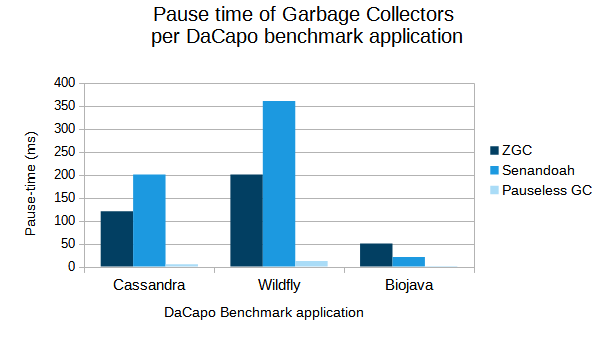
\includegraphics[width=1\columnwidth]{img/graph2.png}
    \end{figure}
\end{graph1section}


\begin{graph2section}
%    \caption{Simulatie van verwachte resultaten van de gebruikte geheugen op piekmoment voor bepaalde Garbage Collectors voor enkele DaCapo benchmark applicaties:}
    \begin{figure}[hbt!]
        \centering
        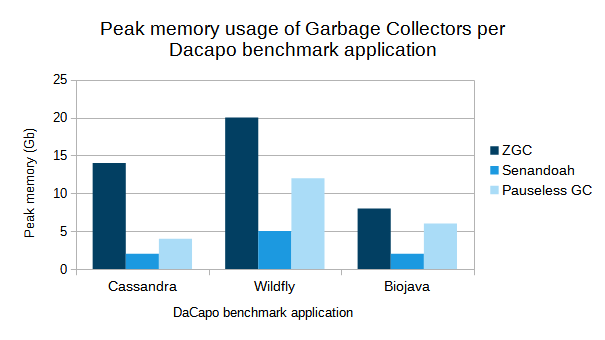
\includegraphics[width=1\columnwidth]{img/graph3.png}
    \end{figure}
\end{graph2section}
%Hier beschrijf je welke resultaten je verwacht. Als je metingen en simulaties uitvoert, kan je hier al mock-ups maken van de grafieken samen met de verwachte conclusies. Benoem zeker al je assen en de onderdelen van de grafiek die je gaat gebruiken. Dit zorgt ervoor dat je concreet weet welk soort data je moet verzamelen en hoe je die moet meten.

%Wat heeft de doelgroep van je onderzoek aan het resultaat? Op welke manier zorgt jouw bachelorproef voor een meerwaarde?

%Hier beschrijf je wat je verwacht uit je onderzoek, met de motivatie waarom. Het is \textbf{niet} erg indien uit je onderzoek andere resultaten en conclusies vloeien dan dat je hier beschrijft: het is dan juist interessant om te onderzoeken waarom jouw hypothesen niet overeenkomen met de resultaten.



%%---------- Andere bijlagen --------------------------------------------------
% TODO: Voeg hier eventuele andere bijlagen toe. Bv. als je deze BP voor de
% tweede keer indient, een overzicht van de verbeteringen t.o.v. het origineel.
%\input{...}

%%---------- Backmatter, referentielijst ---------------------------------------

\backmatter{}

\setlength\bibitemsep{2pt} %% Add Some space between the bibliograpy entries
\printbibliography[heading=bibintoc]

\end{document}
